\documentclass{ucll-slides}
\usepackage{pxfonts}
\usepackage{tikz}
\usepackage{calc}
\usepackage{ucll-code}


\usetikzlibrary{calc,shadows,tikzmark}

\coursename{Distributed Applications}
\title{Processes}

\pgfkeys{
  /envelope/.cd,
  width/.initial=1cm,
  height/.initial=0.8cm,
  position/.initial={0,0},
  value/.initial={},
  value font/.initial={\ttfamily}
}

\newcommand{\envelope}[1][1]{
    {
        \pgfkeys{/envelope/.cd,#1}
        \pgfkeys{/envelope/width/.get=\envwidth}
        \pgfkeys{/envelope/height/.get=\envheight}
        \pgfkeys{/envelope/position/.get=\envposition}
        \draw[fill=white] (\envposition) rectangle ++(\envwidth,\envheight);
        \draw[fill=white] (\envposition) -- ++(\envwidth * 0.5,\envheight * 0.6) -- ++(\envwidth * 0.5,-\envheight * 0.6) -- cycle;
        \draw[fill=white] ($ (\envposition) + (0,\envheight) $) -- ++(\envwidth * 0.5,-\envheight * 0.6) -- ++(\envwidth * 0.5,\envheight * 0.6) -- cycle;
    }
}

\newcommand{\csharp}{C$^\sharp$}

\begin{document}

\maketitle

% \input{aux-os-refresher}
% \section{Elixir Processes}

\begin{frame}
    \frametitle{Warning}
    \begin{itemize}
        \item Elixir abstracts away OS concepts such as processes and threads
        \item It can still be useful to know how exactly Elixir concepts map on OS concepts
        \item {\bfseries\color{red} Elixir reuses same terms but assigns different meaning!}
    \end{itemize}
\end{frame}

\begin{frame}
    \frametitle{Elixir Processes}
    \code[language=elixir]{hello-world.exs}
    \begin{itemize}
        \item In other language
              \begin{itemize}
                \item A \emph{thread} executes this line of code
                \item After this, the thread ends
              \end{itemize}
        \item In Elixir
              \begin{itemize}
                \item A \emph{process} executes this line of code
                \item After this, the process ends
              \end{itemize}
        \item Only difference: terminology
    \end{itemize}
\end{frame}

\begin{frame}
    \frametitle{Thread Creation in \csharp}
    \code[language=csharp,font=\small,width=.95\linewidth]{create-thread.cs}
    \begin{itemize}
        \item New thread needs entry point
        \item Constructor is given function
        \item Thread will call \texttt{ThreadProc}
        \item Thread dies when \texttt{ThreadProc} is done
    \end{itemize}
\end{frame}

\begin{frame}
    \frametitle{Process Creation in Elixir}
    \code[language=elixir,font=\small,width=.95\linewidth]{spawn-process.exs}
    \begin{itemize}
        \item New thread needs entry point
        \item \texttt{spawn} is given function
        \item Process will call \texttt{threadfunc}
        \item Process dies when \texttt{threadfunc} is done
    \end{itemize}
\end{frame}

\begin{frame}
    \frametitle{So What's The Big Deal?}
    \begin{itemize}
        \item Difference between Elixir and \csharp?
        \item Currently limited to aesthetics
        \item What's up with that, Elixir? Why do you even exist?
    \end{itemize}
\end{frame}

\begin{frame}
    \frametitle{Communication Between Threads in \csharp}
    \code[language=csharp,font=\small,width=.95\linewidth]{communication.cs}
\end{frame}

\begin{frame}
    \frametitle{Communication Between Processes in Elixir}
    \begin{center}
        \Huge ...
    \end{center}
\end{frame}

\begin{frame}
    \frametitle{Communication Between Processes in Elixir}
    \begin{itemize}
        \item Elixir is purely functional
        \item There is no state
        \item A newborn process can receive data, but it never changes
        \item Communication is in essence change
        \item There is no way to communicate without state
        \item Are we in trouble?
    \end{itemize}
\end{frame}

\begin{frame}
    \frametitle{Communication Between Processes in Elixir}
    \begin{itemize}
        \item Elixir introduces a tiny bit of state
        \item It's fully handled internally by Elixir
        \item No need for synchronization due to shared state
    \end{itemize}
\end{frame}


\begin{frame}
    \frametitle{Message Passing}
    \begin{center}
        \begin{tikzpicture}[process/.style={drop shadow,fill=red!50},
                            process header/.style={black,opacity=0.5},
                            mailbox/.style={drop shadow,fill=blue!50}]
            \begin{scope}
                \coordinate (process a center) at (2,2.5);
                \coordinate (process a queue) at (0.25,-0.25);
                \draw[process] (0,0) rectangle ++(4,5);
                \node[process header,minimum width=4cm,anchor=north west] at (0,5) { Process A };
                \draw[mailbox] (0.5,-0.5) rectangle ++(3,1);
            \end{scope}

            \begin{scope}[xshift=4.5cm]
                \coordinate (process b center) at (2,2.5);
                \coordinate (process b queue) at (0.75,-0.4);
                \draw[process] (0,0) rectangle ++(4,5);
                \node[process header,minimum width=4cm,anchor=north west] at (0,5) { Process B };
                \draw[mailbox] (0.5,-0.5) rectangle ++(3,1);
            \end{scope}

            \only<2>{
                \node[font=\tt] at (process a center) {
                    send(B, :hello)
                };
            }

            \only<3>{
                \node[font=\tt] (send) at (process a center) {
                    send(B, :hello)
                };

                \envelope[position=process b queue]

                \draw[-latex,ultra thick] (send) -- ($ (process b queue) + (0,0.4) $);
            }

            \only<4>{
                \node[font=\tt] (receive) at (process b center) {
                    receive
                };

                \envelope[position=process b queue]
            }

            \only<5>{
                \node[font=\tt] (receive) at (process b center) {
                    receive
                };

                \envelope[position=process b queue]
                \draw[-latex,ultra thick] ($ (process b queue) + (0.5,0.4) $) -- (receive);
            }
        \end{tikzpicture}
    \end{center}
\end{frame}

\begin{frame}
    \frametitle{Message Passing}
    \code[language=elixir,font=\small]{message-passing.exs}
\end{frame}


\end{document}

%%% Local Variables:
%%% mode: latex
%%% TeX-master: t
%%% End:
